%===============================================================================
% LaTeX sjabloon voor de bachelorproef toegepaste informatica aan HOGENT
% Meer info op https://github.com/HoGentTIN/bachproef-latex-sjabloon
%===============================================================================

\documentclass{bachproef-tin}

\usepackage{hogent-thesis-titlepage} % Titelpagina conform aan HOGENT huisstijl
\usepackage{physics}

%%---------- Documenteigenschappen ---------------------------------------------
% TODO: Vul dit aan met je eigen info:

% De titel van het rapport/bachelorproef
\title{How will quantum computing affect the mainframe environment and its applications?}

% Je eigen naam
\author{Lukas Marivoet}

% De naam van je promotor (lector van de opleiding)
\promotor{Martijn Saelens}

% De naam van je co-promotor. Als je promotor ook je opdrachtgever is en je
% dus ook inhoudelijk begeleidt (en enkel dan!), mag je dit leeg laten.
\copromotor{Francis Harkins}

% Indien je bachelorproef in opdracht van/in samenwerking met een bedrijf of
% externe organisatie geschreven is, geef je hier de naam. Zoniet laat je dit
% zoals het is.
\instelling{---}

% Academiejaar
\academiejaar{2019-2020}

% Examenperiode
%  - 1e semester = 1e examenperiode => 1
%  - 2e semester = 2e examenperiode => 2
%  - tweede zit  = 3e examenperiode => 3
\examenperiode{2}

%===============================================================================
% Inhoud document
%===============================================================================

\begin{document}

%---------- Taalselectie -------------------------------------------------------
% Als je je bachelorproef in het Engels schrijft, haal dan onderstaande regel
% uit commentaar. Let op: de tekst op de voorkaft blijft in het Nederlands, en
% dat is ook de bedoeling!

\selectlanguage{english}

%---------- Titelblad ----------------------------------------------------------
\inserttitlepage

%---------- Samenvatting, voorwoord --------------------------------------------
\usechapterimagefalse
%%=============================================================================
%% Voorwoord
%%=============================================================================

\chapter*{\IfLanguageName{dutch}{Woord vooraf}{Preface}}
\label{ch:voorwoord}

%% TODO:
%% Het voorwoord is het enige deel van de bachelorproef waar je vanuit je
%% eigen standpunt (``ik-vorm'') mag schrijven. Je kan hier bv. motiveren
%% waarom jij het onderwerp wil bespreken.
%% Vergeet ook niet te bedanken wie je geholpen/gesteund/... heeft

Why did I choose to explore the quantum realm without any prior knowledge/ education? Quantum computing is being transformed to a real buzzword much like data science was. The field has been opened up from just highly specialised academics to an open source community willing to teach outsiders the very basics.

Also the mere fact that the field of quantum computing is developing to a profitable and sustainable business so rapidly has astonished me from my very first contact with the environment.

 I would like to thank Frank Harkins from IBM for being available to have a chat about quantum computing and how it will influence our societies and even our very nature of problem-solving. 
 
 But most of all I would like to congratulate the research environment around quantum computing on how accepting and supportive they are for all interested parties. In the next decade quantum computing will only become more apparent and obvious to a point where quantum computing becomes an essential part of problem solving anything within a reasonable time scheme.
 
 So that is exactly why this paper will serve as a great starting tool for a computer scientist that is interested in the multiple ways quantum computers could influence the general sector.

%%=============================================================================
%% Samenvatting
%%=============================================================================

% TODO: De "abstract" of samenvatting is een kernachtige (~ 1 blz. voor een
% thesis) synthese van het document.
%
% Deze aspecten moeten zeker aan bod komen:
% - Context: waarom is dit werk belangrijk?
% - Nood: waarom moest dit onderzocht worden?
% - Taak: wat heb je precies gedaan?
% - Object: wat staat in dit document geschreven?
% - Resultaat: wat was het resultaat?
% - Conclusie: wat is/zijn de belangrijkste conclusie(s)?
% - Perspectief: blijven er nog vragen open die in de toekomst nog kunnen
%    onderzocht worden? Wat is een mogelijk vervolg voor jouw onderzoek?
%
% LET OP! Een samenvatting is GEEN voorwoord!

%%---------- Nederlandse samenvatting -----------------------------------------
%
% TODO: Als je je bachelorproef in het Engels schrijft, moet je eerst een
% Nederlandse samenvatting invoegen. Haal daarvoor onderstaande code uit
% commentaar.
% Wie zijn bachelorproef in het Nederlands schrijft, kan dit negeren, de inhoud
% wordt niet in het document ingevoegd.

\IfLanguageName{english}{
\selectlanguage{dutch}
\chapter*{Samenvatting}

Zoals het onderzoek aantoont, staat onderzoeksgebied van kwantum computers nog in zijn kinderschoenen en moeten we kritisch blijven ten opzichte van elke nieuwe uitgave in verband met nieuw onderzoek. Echter is het ook belangrijk dat we buiten het puur theoretische deel ook effectief op zoek gaan naar de praktische toepassingen en/ of inzichten in onze huidige processen met evt. de toepassing van kwantum verwerking in deze bestaande processen. 

In het onderzoek proberen we een duidelijk beeld weer te geven aan de lezer, zodat hij/ zij zelfstandig kan nadenken over toepassingen en/of zelf toevoegingen kan maken aan de vele 'open source' gemeenschappen op Github. Dit hebben we proberen te bereiken door enkele praktische weergaves te maken met de hulp van het Python-framework Qiskit over de uitvoering op een kwantum systeem. De resultaten wijzen er inderdaad op dat we bestaande problemen ook kunnen oplossen met kwantum algoritmes, maar zoals te zien aan de werkelijke uitvoeringen op de echte kwantum computers van IBM is het moeilijk om deze nieuwe technologieën al meteen toe te passen in bestaande productiesystemen. 

In de paper is er ook een focus gelegd op de mogelijke samenwerking van de mainframe in het verhaal over kwantum computers. De verwachtingen zijn al enorm over de samenwerking tussen onze huidige supercomputers en een kwantum systeem, maar dit betekent dus ook dat er een enorm potentieel bestaat tussen een mainframe machine en een kwantum systeem. De potentiële winst van kwantum wordt voorzien in enorme versnellingen van data verwerkingen en dat is nu exact waar een mainframe machine zo krachtig is; het genereren van enorme hoeveelheden data.

Om er zeker van te zijn dat de lezer een volledig beeld krijgt van dit interessante onderwerp, wordt er gezorgd dat kwantum computers van alle kanten worden bekeken.



\selectlanguage{english}
}{}

%%---------- Samenvatting -----------------------------------------------------
% De samenvatting in de hoofdtaal van het document

\chapter*{\IfLanguageName{dutch}{Samenvatting}{Abstract}}

The field of quantum computers is still in its infancy and we must remain critical of any new publication related to new insights. However, it is also important that beyond the purely theoretical part, we also effectively look for practical applications and/or insights into our current processes with the possible application of quantum processing in them. 

During research we tried to present a more clear picture to the reader, so that he or she can independently think about applications and/or make additions to the many open source communities on Github. We have tried to achieve this by making some practical showcases with the help of the Python framework Qiskit for quantum computing. The results indeed point to the possible execution of quantum algorithms on already existing computer science problems. But as can be seen from the actual results on IBM's real quantum computers, it is difficult to use these new technologies in existing production systems at this point in time. 

In this  research paper there is also a focus on the incorporation of the mainframe in the story of quantum computers. The expectations are heightened about the cooperation between our current supercomputers and a quantum system, but this also means that there is a huge potential between a mainframe machine and a quantum system. The benefits of quantum are mostly expected in huge accelerations of data processing and that is exactly what a mainframe machine is so powerful at; generating huge amounts of data.

There is also a strong emphasis on showing all sides of quantum computing as to make sure the reader has a full picture of the whole field.



%---------- Inhoudstafel -------------------------------------------------------
\pagestyle{empty} % Geen hoofding
\tableofcontents  % Voeg de inhoudstafel toe
\cleardoublepage  % Zorg dat volgende hoofstuk op een oneven pagina begint
\pagestyle{fancy} % Zet hoofding opnieuw aan

%---------- Lijst figuren, afkortingen, ... ------------------------------------

% Indien gewenst kan je hier een lijst van figuren/tabellen opgeven. Geef in
% dat geval je figuren/tabellen altijd een korte beschrijving:
%
%  \caption[korte beschrijving]{uitgebreide beschrijving}
%
% De korte beschrijving wordt gebruikt voor deze lijst, de uitgebreide staat bij
% de figuur of tabel zelf.

\listoffigures
\listoftables

% Als je een lijst van afkortingen of termen wil toevoegen, dan hoort die
% hier thuis. Gebruik bijvoorbeeld de ``glossaries'' package.
% https://www.overleaf.com/learn/latex/Glossaries

%---------- Kern ---------------------------------------------------------------

% De eerste hoofdstukken van een bachelorproef zijn meestal een inleiding op
% het onderwerp, literatuurstudie en verantwoording methodologie.
% Aarzel niet om een meer beschrijvende titel aan deze hoofstukken te geven of
% om bijvoorbeeld de inleiding en/of stand van zaken over meerdere hoofdstukken
% te verspreiden!

%%=============================================================================
%% Inleiding
%%=============================================================================

\chapter{\IfLanguageName{dutch}{Inleiding}{Introduction}}
\label{ch:inleiding}

Why does everyone suddenly jump on the subject of quantum computing \textbf{(QC)} and why would it concern anyone at this point in time? Well we are rapidly reaching the limits of how small we are able to create the transistors on a chip, Moore's Law may very well be about to end. Currently we are able to create transistors so small that they themselves start being influenced by the quantum world which would undermine the whole point of building smaller and smaller components that are faster than its predecessors. \autocite{Hartnett2019}

The quantum field itself is also rapidly expanding due to the practical executions of QC, much in the same way data science has been expanding for the last 2 decades. Only 20 years ago data was something nice to have in a business to gain a possible edge over opponents, now data is the lifeblood for many of those companies. Data is what drives research, competitive advantage and various innovations. QC could offer our way of data handling and processing a surprising speed boost and expansion into regions we just were not able to even understand due to its quantum nature e.g. in sectors like Chemistry, Astronomy, Physics...  And this is exactly why the mainframe environment could tie in so nicely into the research towards a classical and quantum computational combined environment. Mainframes drive the big enterprises who in turn drive the smaller ones that our societies are built upon. If QC could aid these big enterprises they would in turn let this information flow through into the lower sectors of our global economy. All this is why the paper will try and expose why we should start noticing about QC in the very same everyone suddenly started keeping track of data research with classical computing.~\autocite{Google2019} ~\autocite{IBM2019}


\section{\IfLanguageName{dutch}{Probleemstelling}{Problem Statement}}
\label{sec:probleemstelling}

What can QC actually solve as of this very moment, is a question every interested enterprise is trying to figure out first. The field has shown even in this very early state with the limited amount of computational resources much promise. Inside the fields of data processing there is a clear trend that as we further develop quantum computational expertise the possible business impacts are generated exponentially. Many big enterprises have finally figured out the most lucrative and easy-to-apply ways of capturing important data that could have business value. Now the actual issue that most definitely is worth addressing, is that the processing of the shear amount of data has become unbearable in realistic time schemes. 

Business needs all these data results as soon as possible to gain the edge over competitors and industry leaders. Quantum could in theory exponentially aid classical computers with the processing of this large amount of data. Mainframes especially are able to generate so much I/O with all sorts of data e.g. credit card spending, production analysis, transport optimization, that the mainframe together with QC could very well become the power couple of the 21st century. With platforms as Qiskit and Cirq everyone is able to contribute towards quantum research even within a mainframe minded environment.  ~\autocite{Qiskit} and ~\autocite{Cirq}

\section{\IfLanguageName{dutch}{Onderzoeksvraag}{Research question}}
\label{sec:onderzoeksvraag}

The question of "How will QC affect the mainframe environment and its applications?" can be a really useful question to solve because it would allow the highly expertised environment of the mainframe to be able to think of possible applications of the quantum research with their mainframe systems. In this moment of time practical QC has come such a long way that this question could possibly give added business value to the mainframe industry and all of their users. Exploring this domain can provide valuable insights in all different kinds of sectors that make use of the mainframe's high-data capabilities.

\section{\IfLanguageName{dutch}{Onderzoeksdoelstelling}{Research objective}}
\label{sec:onderzoeksdoelstelling}

The paper is designed to allow individuals that are interested in QC and general computer science  to get a better grasp on the real business impacts of the quantum realm. We expect that we can evaluate the real value of QC inside a business, but also we want to find actual value and applications inside the sector as a whole. Following up with the real practical showcase of these new quantum technologies using a Python framework that is freely available for anyone to download and use. The framework is called Qiskit and is at the moment of writing the only framework that allows the connection to real quantum devices. This connection is free of charge, where you are able to create quantum circuits and test them out on simulators of the framework  itself to then follow these circuits up by sending them off to a quantum device and get back the results from it. By being able to look at real executions you instantaneously receive a better grasp of the whole aspect of quantum phenomena.

\section{\IfLanguageName{dutch}{Opzet van deze bachelorproef}{Structure of this bachelor thesis}}
\label{sec:opzet-bachelorproef}

The paper will consist of the following chapters:

In chapter ~\ref{ch:quantum-essentials}, we will introduce the very basic usage of QC to make sure every reader is able to understand the basic necessary principles to understand this paper.

In chapter ~\ref{ch:computing-with-quantum}, we will expose how classical and QC could offer a valuable partnership in their effort to speed up all research. 

In chapter ~\ref{ch:practical}, we will finally show the real usages of quantum algorithms of the future through simulations or even executions on real devices with Qiskit. The algorithm that we will use will be an adaptation of Grover's algorithm for a unstructured search, more specifically an algorithm that is able to solve the 3-SAT problem in an advantageous manner.

This chapter will be designed for computer scientist that want to really understand the technology and want to learn and maybe even contribute themselves towards the many open source options out there surrounding QC.

In chapter~\ref{ch:conclusie}, there will be an extensive discussion where we take in the results of the practical compartment of this paper. Furthermore we would still like to take a critical look at how QC has its benefits but also its disadvantages. 
\chapter{\IfLanguageName{dutch}{Stand van zaken}{Quantum Essentials}}
\label{ch:quantum-essentials}

To make sure everyone starts from the same baseline to understand the full potential of this paper, we will introduce a few of the basic quantum principles. This paper is not targeting these specific principles but does use them to explain different practical consequences of the use of them within quantum computation. If there is any further interest regarding these principles, we would refer you to the following papers, ~\textcite{Rieffel1998} and ~\textcite{Shor2000}.

\subsection{The Qubit and its classical opponent}

The foundation of any quantum related paper is and will always be the \textbf{qubit}. A qubit is just like a classical computing bit the foundational unit of its computer. Whilst a bit can either be on or off, a qubit has a certain statistical measurement to it. To be able to program on a quantum computer you need to think of the issue of computing an equation in a completely different way. A qubit is also not infinite, meaning that any type of computation needs to happen during the time frame of stable qubit without being thrown of its state by decoherence or any other external factors. 

During the execution of your program you are simply not able to look at the intermediary results as this would affect the final result, which would make the whole computation worthless. This means that debugging and looking at variables whilst you are executing a piece of code simply is not possible, which in turn makes writing actual code for a quantum computer a lot more difficult. 

To comprehend the nature of a qubit we need to understand that representing a qubit is only possible in a complex field, which shows of a certain amplitude of the state of the qubit in a point in time. \textit{Felix Bloch} was the individual that came up with the Bloch sphere that we currently use to clearly represent what a qubit is at a certain point in time. 

To sum it up a bit can be only be in a state of on or off and this can be checked throughout execution, whilst a qubit is in a uncertain state during execution much like Schrödinger's cat but once observed is just as determined as a normal bit would be. But determining the state during execution will affect the rest of the experiment and will remove the advantage of quantum in much the same way if Schrödinger went on with the experiment after observation that the cat died, he would be certain that cat would still be dead at a later point.

\begin{figure}[h]
\centering
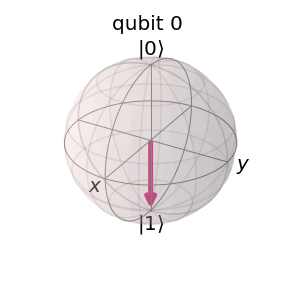
\includegraphics[scale = 0.75]{../Demonstration/img/Quantum_essentials_1.PNG}
\caption{A Bloch sphere representation of 1 qubit in the |1> state. The Bloch sphere clearly indicates that the state of a qubit has a certain probabilistic aspect to it.}
\end{figure}

\subsection{Superposition and entanglement}

\textbf{Superposition} is a term a lot of people have heard about and how it could achieve major breakthroughs in the scientific world, but what does it exactly represent is the real question. Quantum advantage is mostly gained from this quantum principle, where a quantum particle can remain in both states at once whilst it has not been observed. To explain this more clearly from a computer science angle, a qubit in superposition is during execution behaving as 0 and 1 at the same time. A concept that seems impossible within a classical frame of mind but also very advantageous if you know where to look. To put it more clearly, e.g. if you are processing a big array of data through your processor, your processor will take one item of the array, process, convert and output it before it will take another item of the array and perform the same thing. A quantum computer could go about this process in a similar yet much more ingenious way. A quantum processor would put an amount of qubits in superposition to represent the array as input, perform the needed amount of quantum gates and receive the output in a single go instead of needing to loop over the full array. ~\autocite{Draper2000}

\textbf{Entanglement} is another major principle within the realm of quantum physics. It refers to the correlation between entangled qubits where the state of one qubit influences the state of the correlated qubit in a way that it can be exploited theoretically infinitely speed up computation. This entanglement can be achieved inside a quantum computer by the use of quantum gates on qubits in a state of superposition. The deterministic result of the qubits at the end of an experiment will show the same correlation in the results, keeping in mind that enough experiments are performed to defend against quantum decoherence mistakes and other external influences.
~\autocite{fern2016mathematics}

These two principles are constantly being used  by a quantum processor as the one that Google showed of in their latest showcase of their quantum supremacy, ~\textcite{Google2019}. Together they are able to exponentially increase the computing power of a quantum computer, as you add more and more qubits you are exponentially increases the available data items such a processor could handle. For example to be able to simulate the biggest medicine of the 20th century, penicillin you would need 286 functional qubits, which in turn would be able to generate the $2^{286}$ bits of memory. This amount of memory is impossible to be able to achieved with a classical amount of bits, while a quantum computer in turn would be able to complete the simulations with theoretically 286 stable qubits. Actually getting to such a stable amount of qubits in itself will still be a scientific miracle. 






%%=============================================================================
%% Methodologie
%%=============================================================================

\chapter{\IfLanguageName{dutch}{Methodologie}{Computing real-world solutions with Quantum}}
\label{ch:computing-with-quantum}

%% TODO: Hoe ben je te werk gegaan? Verdeel je onderzoek in grote fasen, en
%% licht in elke fase toe welke stappen je gevolgd hebt. Verantwoord waarom je
%% op deze manier te werk gegaan bent. Je moet kunnen aantonen dat je de best
%% mogelijke manier toegepast hebt om een antwoord te vinden op de
%% onderzoeksvraag.

\lipsum[21-25]


%%=============================================================================
%% Methodologie
%%=============================================================================

\chapter{Practical demonstration with Qiskit}
\label{ch:practical}

For two decades now people have been receiving fully blown quantum mechanics courses where they are able to experiment with the thought of quantum experiments in a theoretical type of way, but never were truly interested parties able to perform their experiments in a free and fluid manner. QC is at a point where we are able to effectively experiment with the technology as a broader community. Platforms like Qiskit are excellent in their reach towards interested parties and are more than welcoming towards new developments that could aid the whole community in its research and adaption. The service is open source which truly pushes the whole movement of research out of this shroud of high costs and large enterprises. This will obviously influence other branches to follow in the same footsteps as to allow every party that is interested or has a passion to be able to participate in a costless and open manner. To remain objective and fair towards other companies outside of IBM, Google is also participating in the open source community with platforms like Cirq, \textcite{Cirq}. 

In the following part, we will lay out how any interested parties are able to perform their own executions on real devices and start applying what some of them have been learning theoretically for over 20 years.

\subsection{Grover's search algorithm in a practical fashion}
\subsubsection{Grover's search unstructured database search}

We have chosen for an adaptation of an algorithm that could prove extremely useful for any implementation together with a mainframe, which is the Grover Search algorithm applied for the boolean satisfiability problem. The whole premise of the original algorithm is that we are able to speed up the search time in an unstructured database. This all meaning when a computer needs to find an item with an unique attribute that differentiates itself from the other items in the list, QC could become the main solution to a brute force task like that. The whole algorithm uses something called "amplitude amplification" where the algorithm influences the probabilities in such a manner that the specific item has the highest probability after the quantum computation. \autocite{Grover1996}

To clarify amplitude amplification further, this is a principle that affects qubits in their superposition and entangled states where they would interfere with each other to eliminate the least likely outcomes and amplify the statistical chance of the desired item. By applying this to an algorithm after the correct transformations, you would be able to decompose all the different results back to a highly probable result that does not collapse all the qubits in superposition like any normal measurement would. 

\subsubsection{Grover's search algorithm in an applied form}

For the experiment itself, we have chosen for the specific "Boolean satisfiability problem" which uses Grover's way of amplitude amplification to find the correct results of a boolean problem. This computer science question goes as follows, given a boolean comparison of multiple parts are we able to determine the outcome of this function to where the result of the boolean calculation equal TRUE. Being able to solve this comparison in a single execution could abuse the fact of superposition and entanglement and could prove useful when we scale out the problem towards thousands or even millions of factors for other functions. For now the 3-SAT problem has been chosen to be performed using Qiskit to show off the performance of QC that is available to us.

You are able to view the boolean function in figure 4.1 as the problem that we will try and solve using Quantum technology. The algorithm now needs to find which solutions are possible by interchanging x,y,z with TRUE/FALSE.

\begin{figure}
	$ f(x,y,z) = (\neg x \vee y \vee \neg z) \wedge  ( x \vee \neg y \vee \neg z) \wedge ( x \vee \neg y \vee  z) \wedge (\neg x \vee \neg y \vee z) \wedge  ( x \vee y \vee  z)	 $
	\caption{The 3-SAT problem that we have processed manually, using the quantum simulator and using the real quantum device.}
\end{figure}

				 
\subsubsection{Executing the quantum algorithm}				 

Using a simulator of an ideal quantum computer we are able to show the results in figure 4.2. The probabilities have been amplified to where there are multiple results for this boolean expression. Figure 4.3 shows the gathered results when we sent off the identical circuit towards one of IBM's real quantum devices (IBMQMelbourne16 in this case). 

\begin{figure}[h]
	\centering
	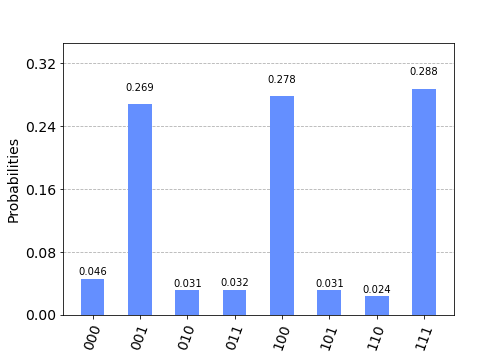
\includegraphics[scale = 0.75]{../Demonstration/img/simulated_3SAT.PNG}
	\caption{These are the results of executing the algorithm for the 3-SAT problem on a \textbf{quantum simulator} that comes with Qiskit. The encoding refers to the TRUE/FALSE value of the x,y,z respectively}
\end{figure}


\begin{figure}[h]
	\centering
	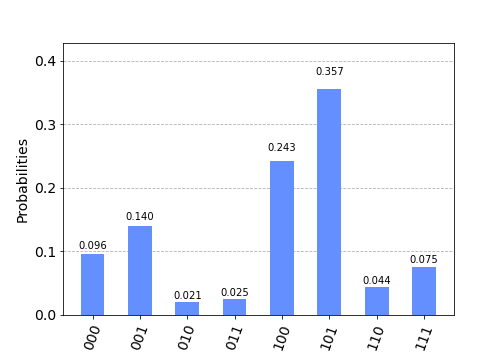
\includegraphics[scale = 0.75]{../Demonstration/img/real_device_3SAT.PNG}
	\caption{These are the results of executing the algorithm for the 3-SAT problem using 15 qubits on a \textbf{real quantum device} that comes with Qiskit. The encoding refers to the TRUE/FALSE value of the x,y,z respectively}
\end{figure}

The reason for choosing this specific experiment is to show that even problems that just require us to encode boolean statements we needed 694 quantum gates. IBMQ transpiles the sent-off circuit to the necessary amount of gates needed for this specific calculation. It does not keep in account that having this much gates on a single line of computation invites a multitude of quantum decoherence issues during runtime. (Appendix A)

Comparing figures 4.2 and 4.3, you are able to see that decoherence for now breaks the probabilities of a computation too much to reliably trust any computation of this size out of a quantum computer. The values became distorted over time by all types of interference.

\begin{table}
	\centering
	\begin{tabular}{|| c c ||}
		\hline
		$f(x,y,z)$ & TRUE/FALSE \\
		\hline\hline
		0 0 0 & FALSE \\ 
		0 0 1 & TRUE \\
		0 1 0 & FALSE \\
		0 1 1 & FALSE \\
		1 0 0 & TRUE \\
		1 0 1 & FALSE \\
		1 1 0 & FALSE \\
		1 1 1 & TRUE \\
		\hline
	\end{tabular}
\caption{These are the results of our 3-SAT problem, calculated in a manual classical manner.}
\end{table}

If we compare the manually gathered results from table 4.1 above across the simulated version and the real version, we are clearly able to see that decoherence has played too big of a role to be certain of any reliable output for these types of large computations. By having these big differences in results we once again prove that simply adding qubits will not be helpful for the reliability in QC. The results differ too much to ever use these results in business cases where speed is as critical as accuracy in reporting towards externals.

Let us work out a clear example (figure 4.4) to make sure our probabilities generated by the real quantum device are incorrect. If we take the highest probability of the real execution which is the configuration of $101$. Meaning that the quantum computer determined that when X and Z are true the whole boolean expression will result in a returned value of TRUE. This is simply not a valid option for this boolean expression. If we look at the first part of this boolean expression we can see that this configuration would return a FALSE resulting in the whole expression being FALSE because all the parts are connected with a logical AND. 

\begin{figure}
	\centering
	$f(1,0,1) = (0 \vee 0 \vee 0 \vee) \wedge (1 \vee 1 \vee 0)  \wedge ( 1 \vee 1 \vee  1) \wedge ( 0 \vee 1 \vee 1) \wedge  ( 1 \vee 0 \vee  1)$
	\caption{The filled-in example for showing how performing this boolean equation on the real device has been influenced too much by quantum decoherence.}
\end{figure}



\subsection{Data-encoding in QC}

As the experiment shows we are able to use quantum algorithms to solve classical computer problems. Of course quantum decoherence has played a great part in the computation and solving it would be greatly beneficial for the whole sector, but there is also a different problem that arises with defining our classical way of problems in a quantum way. The way we represent data in a quantum circuit quickly becomes overly complicated for any large database structure. This is visible from appendix A, where you are able to see how many gates were needed to perform this rather small boolean equation. (694 gates)

So for now quantum computers are not as powerful as classical machines in the way they are able to solve classical problems. But they can have value in the sectors that are the most halted by the use of classical devices. E.g. using them for use-cases like simulating quantum effects we can easily imagine that using a qubit to actually simulate quantum effects is way more effective than simulating a qubit using classical bits.

The issue lies in the fact that we want to input classical database structures/ data-items into a quantum device and hopefully receive the results in a readable classical solution. So if we want to solve existing classical problems we need to find a performant manner of encoding these problems in a quantum device. As appendix A shows, we would need 694 quantum gates to encode and solve this small boolean problem. The generation and application of these gates itself bring a lot of potential decoherence and risk in the reliability of the results, which in turn downgrade the experience of working with the quantum devices as of now.

All of this shows an issue we are facing with the encoding of our classical data to quantum data and back. For the proof-of-concept experiments it does not matter as the encoding time does not influence the runtime of the experiment as a whole. On a normal classical machine, it took 2 seconds to solve this boolean expression and on the quantum device the execution was 7.3 seconds. But once we start scaling out the issue where we would want to find a specific item through the use of Grover's algorithm, we would run into the issue that the encoding and decoding of the input and output could take up a great amount of computational time. If however QC develops in such a way that we are able to gain the full benefits of qubits in superposition, this encoding time could be overcome. But for now it remains a crucial factor in solving the whole feasibility of QC.



\subsection{Mainframe computing with QC}

As the paper has previously stated having QC together with the power of a mainframe could become extremely advantageous for the whole industry to provide the power of data crunching this immense layer of internal data that companies have collected over the years with their mainframes. So we needed to find a circuit that could show off where quantum computing indeed could benefit in the crunching of data in a better/ faster way than classical computing can at the moment. Soon it became clear that simulating anything of a mainframe is impossible for now, we can simulate how a new form of database search could work with Grover. But we are not able to simulate the main advantage of a mainframe device, which is performing quick, stable and secure input and output transformations. And as shown by the experiment it is obvious that having a stable output of a specific input is not one of the main strengths of QC for now. Then when we take into account the encoding and decoding of classical computations and problems it only decreased the feasibility for running mainframe-sized data-sets.


So for now there is no clear advantage when we would use the current developments of QC with the existing mainframe technology, because as stated above we ran into the issue of data-encoding. The potential for QC and mainframe to still become the data-crunching powerhouse of the future is still there. But for this potential to become viable, a couple of major hurdles have to be overcome first.


\subsection{Future prospects}

As for now we are able to play around with the greater problems of quantum computing but to be able to \textit{reliably} solve real-world solutions in a beneficial way remains an uncertainty.

With the current state of engineering, computer scientists will have to wait to fully utilise the system in a reliable fashion. But as engineering develops the power of quantum computing will increase exponentially as stated by Neven's law \autocite{Hartnett2019} with each added qubit to the system, which would make algorithms like this extremely valuable for data-crunching. When we find a way to circumvent the interference of quantum decoherence and the data-encoding issue, a quantum system could become an essential tool for every sector willing to innovate. 



%%=============================================================================
%% Conclusie
%%=============================================================================

\chapter{Discussion}
\label{ch:conclusie}

Quantum computing will most definitely become one of the great buzzwords of the next decade. With the release of \textcite{Google2019} around their interpretation of 'Quantum supremacy', the whole field was catapulted to the forefront of research. All big players in Quantum research have been given a tremendous spotlight for the future of profitable quantum computing. And this is precisely why we need to make the concept more approachable for anybody interested.

\subsection{Quantum computing for now}

Firstly, after thorough research, a couple of interesting conclusions can be drawn. Beginning with one of the most important ones, Quantum computing is here to stay. The technology has given too much promise in too many sectors that have a strong financial backbone. At this point it is important to understand that the world around us that is visible with the naked eye is completely homogeneous with the 'quantum world', meaning that all research to exploring our world around us, can only prove to be profitable in the future.

Secondly returning to the more concrete conclusions of this paper. While executing this specific version of Grover's algorithm, there was a clear trend visible between the theory and the practical example that does show there are some growing pains that come with the expansion of our quantum devices.
Yes, the theory can be fully implemented at this point to visualise its results when we would work in the most perfect of environments like a simulator. But this perfect environment simply does not exist. Meaning that we will have to be creative to reach this edge of perfect conditions to get to a point that these simulated algorithms can become reliable and profitable towards the future. There are two ways of trying to fix the issue of quantum decoherence. Firstly we could create devices that are not influenced by any internal/ external interferences. They could provide a stable platform for algorithms like Shor's encryption breaking algorithm \textcite{gidney2019factor}. The other option would be to account for these interferences to happen anyway and try and compensate them in a software way, much in the same way a computer does error correction for downloaded files. The latter seems to be the more reasonable option where we are already trying to implement these quantum error correction in to provide better results \autocite{Cory1998}. For now there is no clear technique behind the whole principle except to play around with the length that a qubit needs to stay in its elevated $\ket{1}$ state and the length of the circuit as a whole

But this can all be tried out. Because at the moment we are able to extensively experiment with real or simulated quantum devices. There is a multitude of platforms available, most of them are open-source and free to contribute to them as you want to expand their feature-set. Frameworks like Qiskit allow users to design quantum circuits and test them using their built in simulators, which are easy to pick up but hard to master. As of now IBMQ is the only service that allows you to push up your circuits to really test them on a real device owned and managed by IBM. By granting people the privilege to experiment around with the real devices and notice the shortcomings through raw data results, really shows off how dedicated the whole community of computer science is on pushing this technology to the forefront.


\subsection{Quantum computing and its myths}

As shown in the experiment, QC will not change our entire world in the next year in any drastic manner. So theories that quantum computing could break our entire encryption standard in a matter of years seem absurd once you look at the real executions of these needed algorithms on real quantum devices.
Nevertheless we do want to work proactively to have solutions ready-to-go once these machines do become powerful enough to brute force the RSA-encryption by finding the factors of the prime numbers that represent the private keys of encrypted files.
Some researchers also believe that quantum decoherence will prove to be an unpassable obstacle the more qubits we start adding to the systems. This obstacle is the fact that adding more qubits to a system will always increase the internal interference exponentially and thus generate too much decoherence. This indeed is a major hurdle that needs to be overcome to make quantum computing the new standard for solving really hard to solve problems in the computer science community.

\subsection{Quantum computing as an addition}

The one thing we should take away from the dawn of quantum computing the following decade, is that quantum computing is not the one solution for every single issue in computing. It has its advantages and disadvantages just like classical computing. We should strive to make these two technologies as complementary as possible so that they can cancel out each others disadvantages and amplify their advantages. 

With this work, we have tried to inspire people to learn more about the subject of quantum computing and to hopefully entice them into writing their own 'Hello-world-Applications' on any of the freely available frameworks. For the actual executions and setup of the used experiments, we refer to appendix A.

\subsection{Future works}

The potential powerhouse of a mainframe device and a quantum computer can still prove to be advantageous in future works. If IBM keeps up with doubling its pace of releasing quantum computational resources into the world each year, there may be a chance that mainframes and QC prove to be viable in the near future. Also quantum error correction needs to evolve to an acceptable percentage to where we could start thinking about implementing QC machine learning algorithms in our mainframes or even the speeding up the database structures in the devices by using algorithms like Grover's. But for now QC and mainframe are not able to cooperate in an useful manner to add more business value. 

It is useful to explore these options upfront so that we know when the time comes to expand QC towards the mainframe we have a clear scope to all the potential applications of these two devices.


\begin{figure}[h]
	\centering
	
\includegraphics[scale = 0.75]{../Demonstration/img/qiskit_logo.PNG}
	\caption{The platform we used for executing the 3-SAT algorithm on a real quantum device. © Copyright 2020, Qiskit Development Team Last updated on 2020/05/14.}
\end{figure}




%%=============================================================================
%% Bijlagen
%%=============================================================================

\appendix
\renewcommand{\chaptername}{Appendix}

%%---------- Onderzoeksvoorstel -----------------------------------------------

\chapter{Research Proposition}

Under this section you are able to view the original proposition for this paper to introduce the subject with schooling officials and technical promotors. 
This section can also serve as an introduction to this paper for any further interested readers.

To address the whole reason why this paper was created, the subject has become more and more influential in the Computer Science world.
We have officialy come at a point where we are able to think of real world utilisations of quantum computers to further our research in various subjects.
Quantum has become a buzz word at this point, but not everyone that throws it around has a real grasp on what it exactly means.
That is why this paper has been created to aid interested people in the subject to gain a real understanding of what quantum actually is and what it can do.




% Verwijzing naar het bestand met de inhoud van het onderzoeksvoorstel
%---------- Inleiding ---------------------------------------------------------

\section{Introduction} % The \section*{} command stops section numbering
\label{sec:introductie}

With the approaching realisations of quantum technology, the interest in the subject has risen exponentially. There has been a strong believe in the last 30 years that quantum computing can and will influence our environment more than we think. The mainframe environment is one of the sectors that can become the most influential in \emph{computer science}, because of its immense creation of data. Data will become the driving factor inside our societies, think of how much our daily lives are controlled by data ( e.g. online shopping, social media etc.). With the usage of mainframes we are able to create a sense of logic in this almost infinite pile of data. But through the utilisation of quantum computing, data exploration and mining can become much more thorough and meaningful for business applications. The main driving factors for technological breakthroughs have always been wars and economics ( e.g. Atomic energy, commercial aircraft, radio etc.). The more applications of quantum computing that we are able to find for existing economical applications, the more general investment in research will be made. Which would obviously boost both fields at once. In this paper we will try and find these general applications in reality of quantum computing.

\subsection{Topics}
\begin{itemize}
  \item Security implications with the rise of quantum computing
  \item Efficiently exploring mainframe data using quantum computing
  \item Advantages and disadvantages of combining classical computing with quantum computing
  \item Building quantum software before the creation of the hardware
\end{itemize}

%---------- Stand van zaken ---------------------------------------------------

\section{State-of-the-art}
\label{sec:state-of-the-art}
\subsection{Prior knowledge}
Inside the paper a couple of physics associated terms will be utilised. If you are not familiar with basic quantum physics notations, it would be highly recommended to read one or both of the following papers, ~\textcite{Rieffel1998} or ~\textcite{Shor2000}. It is also possible to read this paper as an informational piece without the implications of the mathematics and physics surrounding the subject. As previously stated the paper will not be going in depth technologically, because the paper wants to expose the practical usages of quantum computing compared to classical computing and because that would reach far out of the scope of this paper.

\subsection{Literature review}

As of now Google has claimed to have won the \emph{Quantum Supremacy race} ~\autocite{Google2019}
% Voor literatuurverwijzingen zijn er twee belangrijke 

Je mag gerust gebruik maken van subsecties in dit onderdeel.

%---------- Methodologie ------------------------------------------------------
\section{Methodology}
\label{sec:methodologie}

Hier beschrijf je hoe je van plan bent het onderzoek te voeren. Welke onderzoekstechniek ga je toepassen om elk van je onderzoeksvragen te beantwoorden? Gebruik je hiervoor experimenten, vragenlijsten, simulaties? Je beschrijft ook al welke tools je denkt hiervoor te gebruiken of te ontwikkelen.

%---------- Verwachte resultaten ----------------------------------------------
\section{Expected results}
\label{sec:verwachte_resultaten}

Hier beschrijf je welke resultaten je verwacht. Als je metingen en simulaties uitvoert, kan je hier al mock-ups maken van de grafieken samen met de verwachte conclusies. Benoem zeker al je assen en de stukken van de grafiek die je gaat gebruiken. Dit zorgt ervoor dat je concreet weet hoe je je data gaat moeten structureren.

%---------- Verwachte conclusies ----------------------------------------------
\section{Expected conclusions}
\label{sec:verwachte_conclusies}

Hier beschrijf je wat je verwacht uit je onderzoek, met de motivatie waarom. Het is \textbf{niet} erg indien uit je onderzoek andere resultaten en conclusies vloeien dan dat je hier beschrijft: het is dan juist interessant om te onderzoeken waarom jouw hypothesen niet overeenkomen met de resultaten.



%%---------- Andere bijlagen --------------------------------------------------
% TODO: Voeg hier eventuele andere bijlagen toe
%\input{...}

%%---------- Referentielijst --------------------------------------------------

\printbibliography[heading=bibintoc]

\end{document}
